\documentclass[12pt,a4paper]{article}

\usepackage[T1]{fontenc}
\usepackage[utf8]{inputenc}
\usepackage{lmodern}
\usepackage[left=30mm,right=25mm,top=25mm,bottom=25mm]{geometry}
\usepackage[english, ngerman]{babel}
\usepackage[autostyle=true,german=quotes]{csquotes}
\usepackage[onehalfspacing]{setspace}
\usepackage[expansion=false]{microtype}
\usepackage{booktabs}
\usepackage{tabularx}
\usepackage{enumitem}
\usepackage{xcolor}
\usepackage{amsmath}
\usepackage{amssymb}
\usepackage{pifont}
\usepackage{etoolbox}
\usepackage{caption}
\usepackage{float}
\usepackage{graphicx}
\usepackage{tikz}
\usetikzlibrary{positioning,patterns,arrows.meta,fit,decorations.pathreplacing}
\usepackage{pgfplots}
\pgfplotsset{compat=1.18}
\usepackage{sansmath}

% Einheitlicher Stil fuer alle Abbildungen, abgestimmt auf die
% drawio-Zeichnungen in Diagramme/selbsterstellt (weisse Flaechen,
% gleichmaessige duenne Linien, graue Containerbeschriftung)
\tikzset{
    every picture/.style={line width=0.7pt, >={Latex[length=1.9mm, width=1.3mm]},
        execute at begin picture={\sffamily\sansmath}},
    kasten/.style={draw, fill=white, minimum height=0.5cm, inner sep=2.5pt, font=\scriptsize},
    kastengrau/.style={kasten, fill=black!5},
    % Containerrahmen und deren Beschriftung in Grau, Inhalt in Schwarz
    titel/.style={font=\scriptsize, text=black!55},
    alt/.style={draw=black!45},
    neu/.style={draw=black, line width=0.7pt},
    auftrag/.style={kasten, minimum height=0.4cm, inner sep=2pt},
}

\usepackage[backend=biber,style=ieee,urldate=long]{biblatex}
\addbibresource{sycl.bib}
\usepackage{listings}
\lstset{
    language=C++, basicstyle=\ttfamily\scriptsize, columns=fullflexible,
    keepspaces=true, showstringspaces=false, numbers=left, numberstyle=\tiny\color{gray},
    commentstyle=\color{gray!70!black}, keywordstyle=\bfseries,
    breaklines=true, frame=lines, framesep=3pt, aboveskip=6pt, belowskip=6pt,
    literate={ä}{{\"a}}1 {ö}{{\"o}}1 {ü}{{\"u}}1 {Ä}{{\"A}}1 {Ö}{{\"O}}1
             {Ü}{{\"U}}1 {ß}{{\ss}}1 {–}{{--}}1,
}
% Kopfzeile: links der laufende Abschnitt, rechts die Seitenzahl
\usepackage{fancyhdr}
\pagestyle{fancy}
\fancyhf{}
\fancyhead[L]{\small\nouppercase{\leftmark}}
\fancyhead[R]{\small\thepage}
\renewcommand{\headrulewidth}{0.4pt}
\renewcommand{\footrulewidth}{0pt}
\setlength{\headheight}{15pt}
\fancypagestyle{plain}{\fancyhf{}\renewcommand{\headrulewidth}{0pt}}

\usepackage{hyperref}

\hypersetup{
    colorlinks,
    citecolor   = black,
    filecolor   = black,
    linkcolor   = black,
    urlcolor    = black,
    pdftitle    = {SYCL: Portable heterogene Programmierung mit C++},
    pdfauthor   = {Erlind Sejdiu},
    pdfcreator  = {pdflatex},
    pdfproducer = {LaTeX with hyperref}
}

% Tabellen, Abbildungen und Literaturverzeichnis einzeilig
\AtBeginEnvironment{tabular}{\singlespacing}
\AtBeginEnvironment{tabularx}{\singlespacing}
\AtBeginEnvironment{tikzpicture}{\singlespacing}
\captionsetup{font=small, labelfont=bf}
\captionsetup[table]{position=top, skip=6pt}
\AtBeginBibliography{\singlespacing}

% Befund-\u00dcberschriften als kompakte Lauftitel
\makeatletter
\renewcommand\paragraph{\@startsection{paragraph}{4}{\z@}%
    {0.6ex \@plus 0.3ex \@minus 0.2ex}{-0.6em}%
    {\normalfont\normalsize\bfseries}}
\makeatother

% Verweis auf eine Stelle im Quellcode des Anhangs: \stelle{label}{Zeilen}
\newcommand{\stelle}[2]{(\hyperref[#1]{\ref*{#1}, Z.~#2})}

\begin{document}

% ---------------------------------------------------------------------------
% Titelei (Titelseite ohne Seitenanker, danach römische Seitenzahlen)
% ---------------------------------------------------------------------------
\hypersetup{pageanchor=false}
\begin{titlepage}
    \raggedright
    Erlind Sejdiu\\
    106357
    \vspace*{3cm}

    \begin{center}
        {\LARGE\bfseries SYCL\\[0.3em]
        Portable heterogene\\
        Programmierung mit C++\\[0.4em]
        \large Problemstellung, Programmiermodell und Performance-Portabilität\par}
        \vspace{2cm}
        {\large Seminararbeit\\
        der Hochschule Karlsruhe\\
        im Masterstudiengang Informatik\\
        im Wintersemester 2026/27\par}
    \end{center}
    \vfill
    \begin{tabular}{@{}ll}
        Betreuer: & Prof. Dr.-Ing. Holger Vogelsang\\
        Abgabedatum: & 30.11.2026
    \end{tabular}
\end{titlepage}
\clearpage
\hypersetup{pageanchor=true}
\pagenumbering{Roman}
\setcounter{page}{1}

% ---------------------------------------------------------------------------
% Zusammenfassung
% ---------------------------------------------------------------------------
\section*{Zusammenfassung}
\addcontentsline{toc}{section}{Zusammenfassung}
\markboth{Zusammenfassung}{}

Heterogene Rechnersysteme verbinden CPUs mit spezialisierten Beschleunigern wie GPUs, erschweren die Softwareentwicklung jedoch durch herstellerspezifische Schnittstellen, doppelte Codebasen und den Zielkonflikt zwischen Abstraktion und hardwarenaher Kontrolle. Der offene Standard SYCL verspricht eine einheitliche Codebasis in Standard-C++ für Geräte verschiedener Hersteller. Diese Arbeit untersucht, welche Konzepte des SYCL-Programmiermodells bei einer schrittweisen Portierung benötigt werden und ob neben funktionaler Portabilität auch Performance-Portabilität zwischen CPU und GPU erreicht wird.

Dazu wird eine Matrixmultiplikation in fünf aufbauenden Stufen von sequentiellem C++ nach SYCL portiert. Dieselbe Stufenfolge durchlaufen ein 2D-Stencil und eine Reduktion, beide speichergebunden, sodass sich jeder Schritt bei einem rechen- und bei einem speichergebundenen Problem vergleichen lässt. Gemessen wird mit DPC++~7.2 auf einer AMD-CPU und drei NVIDIA-GPUs (RTX~5060~Ti, L40S, H100) im direkten Vergleich zu handgeschriebenem CUDA und den Bibliotheken des Herstellers. Sämtliche Programme laufen ohne Codeänderung korrekt auf allen vier Geräten. Die erreichte Leistung hängt jedoch davon ab, ob Größen wie die Kachelgröße zum Gerät passen und wie gut die verwendete SYCL-Implementierung für das Zielgerät übersetzt. Einfache Programme erreichen 81 bis 108\,\% der CUDA-Leistung, während nachgebildete statt direkt umgesetzte Sprachmittel -- vor allem atomare Gleitkommaoperationen -- bis auf 5\,\% einbrechen. Welche Stufe sich lohnt, entscheidet zudem das Problem. Bei den speichergebundenen Fallbeispielen kosten die bequemen Speichermodelle 23 bis 74\,\% Bandbreite, und allein die selbst gewählte Gruppengröße hebt den Stencil auf der H100 von 81 auf 101\,\% der CUDA-Leistung.

\newpage
\markboth{Inhaltsverzeichnis}{}
\tableofcontents
\newpage
\listoffigures
\listoftables
\markboth{Abbildungs- und Tabellenverzeichnis}{}
\newpage

% ---------------------------------------------------------------------------
% Hauptteil (arabische Seitenzahlen ab 1)
% ---------------------------------------------------------------------------
\pagenumbering{arabic}

% ---------------------------------------------------------------------------
\section{Einleitung}\label{sec:einleitung}
% ---------------------------------------------------------------------------

\subsection{Problemstellung}\label{sec:problem}

Rechenleistung liegt heutzutage in verschiedenen Formen vor. Neben der CPU
stehen in fast jedem Rechner GPUs und weitere Hardware zur Verfügung, die
datenparallele Aufgaben schnell bearbeiten können. Die Software, um diese
Geräte jeweils anzusprechen, variiert jedoch, denn die großen Hardwarehersteller
pflegen eigene Schnittstellen. Für die Softwareentwicklung ergeben sich daraus
drei Probleme.

\begin{enumerate}[nosep]
    \item Herstellerbindung. CUDA läuft nur auf NVIDIA-GPUs
    \cite{nickolls2008cuda}. AMD (HIP \cite{amd_hip}) und Intel (Level~Zero
    \cite{intel_level_zero}) stellen eigene Programmierschnittstellen bereit.
    \item Mehrfache Codebasen. Wer mehrere Hersteller unterstützen
    will, muss mehrere Implementierungen parallel pflegen.
    \item Abstraktion gegen Kontrolle. Offene Alternativen sind
    entweder sehr hardwarenah und aufwendig wie OpenCL
    \cite{stone2010opencl} oder erlauben wie OpenMP-Direktiven \cite{openmp_spec}
    wenig Kontrolle über Speicherhierarchie und Ausführung.
\end{enumerate}

\subsection{Forschungsfrage und Aufbau}\label{sec:frage}

SYCL ist ein offener Standard der Khronos Group, der diese Probleme lösen
will. Mit einem einzigen Quellcode in Standard-C++ soll auf CPUs und GPUs
verschiedener Hersteller dasselbe Programm laufen \cite{khronos2020sycl}
(Abbildung~\ref{fig:codebasen}).

\begin{figure}[htbp]
\centering
\begin{tikzpicture}[
    code/.style={kasten, minimum width=5.8cm, minimum height=0.5cm},
    hw/.style={kastengrau, minimum width=1.35cm},
]
    \node[code] (s) at (0,1.65) {SYCL-Quellcode};
    \node[code] (i) at (0,0.82) {SYCL-Implementierung (DPC++ / AdaptiveCpp)};
    \node[hw] (g1) at (-2.7,-0.05) {NVIDIA};
    \node[hw] (g2) at (-0.9,-0.05) {AMD};
    \node[hw] (g3) at (0.9,-0.05) {Intel};
    \node[hw] (g4) at (2.7,-0.05) {CPU};
    \draw[->] (s.south) -- (i.north);
    \foreach \g in {g1,g2,g3,g4} \draw[->] (i.south) -- (\g.north);
\end{tikzpicture}
\caption[SYCL-Codebasis für mehrere Backends]{Eine gemeinsame SYCL-Codebasis wird auf verschiedene Backends und Geräte abgebildet}
\label{fig:codebasen}
\end{figure}

Ob ein Programm überall läuft, ist jedoch etwas anderes, als ob es überall
schnell läuft. Diese Arbeit untersucht deshalb die folgende Forschungsfrage.

\begin{quote}
Wie adressiert das Programmiermodell von SYCL die drei genannten
Probleme, und erreicht ein schrittweise nach SYCL portiertes Programm neben
funktionaler Portabilität auch Performance-Portabilität zwischen CPU und
GPU?
\end{quote}

\noindent Daraus ergeben sich zwei Teilfragen. (F1) Welche Konzepte des
Programmiermodells werden bei einer Portierung benötigt, und welches der
drei Probleme lösen sie? (F2) Welche Stufen einer Portierung lassen sich
unverändert auf verschiedenen Geräten ausführen, und welche Parameter
bleiben gerätespezifisch?

% ---------------------------------------------------------------------------
\section{Stand der Technik}\label{sec:stand}
% ---------------------------------------------------------------------------

SYCL basiert auf C++17 \cite{khronos2020sycl} und ist zunächst eine
Spezifikation, die von konkreten Compilern und Laufzeitumgebungen umgesetzt
wird. Die beiden wichtigsten Open-Source-Implementierungen sind DPC++ und
AdaptiveCpp. DPC++ ist eine LLVM-basierte
SYCL-Implementierung von Intel, die neben
Intel-Hardware über entsprechende Plugins auch NVIDIA- und AMD-GPUs unterstützt
\cite{intel_llvm, reinders2023dpcpp}. AdaptiveCpp (ehemals hipSYCL) ist eine
herstellerunabhängige Implementierung der Universität Heidelberg, die
Gerätecode in einem einzigen Compiler-Durchlauf für verschiedene Backends
erzeugt \cite{alpay2020hipsycl, adaptivecpp, alpay2023sscp}. Beide bilden
den Standard über Backends wie CUDA, HIP, Level~Zero, OpenCL oder OpenMP auf
die Zielhardware ab und übersetzen den Gerätecode meist erst beim ersten
Start just in time für das konkrete Gerät \cite{alpay2023sscp}.

SYCL verfolgt vier Entwurfsziele, nämlich Portabilität, Offenheit,
Produktivität und Kontrolle. Tabelle~\ref{tab:vergleich} ordnet
SYCL entlang dieser Ziele ein. Kokkos \cite{edwards2014kokkos} und RAJA
\cite{beckingsale2019raja} verfolgen ähnliche Ziele als C++-Bibliotheken, sind
aber kein offener Industriestandard.

\begin{table}[htbp]
\centering
\small
\newcommand{\ja}{\ding{51}}
\newcommand{\nein}{--}
\newcommand{\teils}{(\ding{51})}
\caption[SYCL im Vergleich zu anderen Programmiermodellen]{SYCL im Vergleich zu anderen Programmiermodellen ((\ding{51}) = eingeschränkt)}
\label{tab:vergleich}
\begin{tabular}{@{}lcccc@{}}
\toprule
 & herstellerunabh. & offener Standard & Standard-C++ & Kontrolle \\
\midrule
CUDA            & \nein   & \nein   & \teils & \ja \\
OpenCL          & \ja     & \ja     & \nein  & \ja \\
OpenMP-Offload  & \ja     & \ja     & \ja    & \teils \\
Kokkos/RAJA     & \ja     & \nein   & \ja    & \teils \\
SYCL            & \ja     & \ja     & \ja    & \ja \\
\bottomrule
\end{tabular}
\end{table}

Eingesetzt wird SYCL vor allem im wissenschaftlichen Rechnen auf Systemen
verschiedener Hersteller, etwa auf dem Supercomputer Aurora oder in GROMACS,
bei der Migration von CUDA-Anwendungen mit dem Werkzeug SYCLomatic sowie in
portablen Bibliotheken wie oneMKL \cite{reinders2023dpcpp}. Frühere Studien
zeigen im Vergleich zu nativem CUDA auf NVIDIA-GPUs, dass SYCL über das
CUDA-Backend für viele HPC- und Lernalgorithmen nahe an die
herstellerspezifische Leistung heranreicht, die tatsächlich erreichte
Geschwindigkeit jedoch deutlich von Implementierung, Codeerzeugung und
Parametrierung abhängt \cite{deakin2020sycl, breyer2022svm}. Für CPUs
beobachten Abram et al.\ \cite{abram2025sycl} zudem erhebliche Unterschiede
zwischen eindimensionalen und mehrdimensionalen Indexräumen bei DPC++ und
AdaptiveCpp. Offen bleibt in diesen Arbeiten meist, welcher Schritt einer
schrittweisen Portierung welchen Effekt auf welchem Gerät hat und an welchen
konkreten Sprachmitteln ein Abstand zu nativem CUDA entsteht. Hier setzt die
vorliegende Arbeit an.

% ---------------------------------------------------------------------------
\section{Methode}\label{sec:methode}
% ---------------------------------------------------------------------------

\subsection{Fallbeispiele}\label{sec:m-fallbeispiele}

Untersucht werden drei Fallbeispiele, die alle dieselbe Stufenfolge der
Portierung durchlaufen (Abschnitt~\ref{sec:m-portierung}). Gegenstand ist nicht
das Rechenproblem selbst, sondern die Veränderung am Programm. Verglichen
wird, was dasselbe Sprachmittel von SYCL bei unterschiedlich gelagerten Problemen
und auf den untersuchten Geräten bewirkt.

Die Stufenfolge wird an der Multiplikation zweier quadratischer Matrizen
entwickelt. Sie führt viele Rechenoperationen auf wenigen Daten aus, ist also
rechengebunden, und lässt sich leicht gegen eine Berechnung auf der CPU
prüfen. Viele praktische Probleme sind dagegen speichergebunden. Sie
rechnen wenig, und ihre Laufzeit wird von der Speichergeschwindigkeit bestimmt.
Dafür stehen ein 5-Punkt-Stencil, der in 100 Zeitschritten die Wärmeausbreitung
auf einer Platte simuliert, indem jeder Gitterpunkt durch den Mittelwert seiner
vier Nachbarn ersetzt wird, und eine Reduktion, die eine lange Zahlenreihe zu
einer einzigen Summe zusammenfasst.

\subsection{Schrittweise Portierung}\label{sec:m-portierung}

Ausgangspunkt ist ein sequentielles C++-Programm auf einem CPU-Kern (Stufe~0).
Jede weitere Stufe nimmt genau eine Veränderung vor und führt nur die Konzepte
ein, die dieser Schritt benötigt (Tabelle~\ref{tab:stufen}).
Kapitel~\ref{sec:konzepte} erklärt sie, der Quellcode steht in
Anhang~\ref{sec:anhang}~(F1). Weil jede Stufe einzeln gemessen wird, zeigt sich,
was jeder Schritt auf jedem Gerät bringt~(F2).

\begin{table}[htbp]
\centering
\footnotesize
\caption[Stufen der Portierung und eingeführte Konzepte]{Stufen der Portierung und die dabei eingeführten Konzepte}
\label{tab:stufen}
\begin{tabularx}{\textwidth}{@{}c>{\raggedright\arraybackslash}X>{\raggedright\arraybackslash}X@{}}
\toprule
Stufe & Änderung & Neue Konzepte \\
\midrule
0 & Sequentielles Ausgangsprogramm auf einem CPU-Kern & -- \\
1 & Die Arbeit wird auf viele parallele Einheiten verteilt & Host und Gerät, Queue, Kernel, Indexraum, gemeinsamer Speicher, Backends, Geräteauswahl \\
2 & Eigener Gerätespeicher, Daten werden ausdrücklich hin- und zurückkopiert & Gerätespeicher, explizite Kopien, asynchrone Ausführung und Abhängigkeiten \\
2b & Wie Stufe~2, aber das Kopieren übernimmt die Bibliothek & Buffer, Accessoren, automatische Abhängigkeiten \\
3 & Die Arbeit wird selbst in Gruppen eingeteilt, noch ohne schnellen Zwischenspeicher & Work-Group und selbst gewählte Gruppengröße \\
4 & Rechnen in Kacheln fester Größe im schnellen Zwischenspeicher der Gruppe & Command Group, lokaler Speicher, Barriere \\
5 & Kachelgröße erst beim Programmstart passend zum Gerät gewählt & Geräteabfragen, nachträglich eingesetzte Konstanten, Fehlerbehandlung \\
\bottomrule
\end{tabularx}
\end{table}

Stencil und Reduktion durchlaufen dieselben Stufen. Bezugspunkt ist dort die
Fassung mit eigenem Gerätespeicher (Stufe~2), die Buffer-Variante (2b) wird je
Messung einmal neu angelegt und einmal wiederverwendet. Bei der Reduktion fallen
die Stufen~3 und~4 zusammen, denn eine selbst gewählte Gruppengröße allein
ändert dort nichts. Erst das Zusammenfassen im lokalen Speicher senkt die
atomaren Zugriffe auf das Gesamtergebnis von einem je Work-Item auf einen je
Gruppe, eine zweite Fassung nutzt dafür ein Gruppenkollektiv. Drei Varianten
haben kein Gegenstück bei den übrigen Fallbeispielen. Beim Stencil lässt sich das
zweidimensionale Gitter auch eindimensional indizieren \cite{abram2025sycl}, und
weil er 100 Zeitschritte nacheinander startet, macht ein Warten der CPU nach
jedem Schritt die Startzeit eines Auftrags sichtbar. Für die Reduktion bietet
SYCL als einziges Fallbeispiel eine fertige Abstraktion.

\subsection{Versuchsaufbau}\label{sec:m-aufbau}

Gemessen wird mit DPC++~7.2 \cite{intel_llvm} auf vier Geräten, einer AMD-CPU
(sechs Kerne) und einer NVIDIA GeForce RTX~5060~Ti in einem Arbeitsplatzrechner
sowie den Rechenzentrums-GPUs L40S und H100 des DACHS-Clusters der Hochschule
Esslingen. Jedes Programm wird je Rechner einmal übersetzt, ohne es auf eine GPU
festzulegen, und läuft dort unverändert auf allen Geräten. Als Vergleich sind die
wichtigsten Varianten aller Fallbeispiele zusätzlich in CUDA umgesetzt, mit
demselben Verfahren und derselben Zeitmessung. Als Obergrenze dienen die
NVIDIA-Bibliotheken cuBLAS \cite{nvidia_cublas} und CUB \cite{nvidia_cub}.
Details zu Hardware, Compilern und Problemgrößen stehen in
Anhang~\ref{sec:messbedingungen}.

\subsection{Messgrößen}\label{sec:m-messgroessen}

Gemessen wird auf der CPU die Zeit von der Übergabe des Auftrags an das Gerät bis
zum Vorliegen des Ergebnisses. Angegeben ist der Median aus fünf Läufen. Der erste
Lauf wird getrennt ausgewiesen, weil in ihm noch der Gerätecode erzeugt wird
(Abschnitt~\ref{sec:k-grundlagen}). Jedes Ergebnis wird gegen eine Berechnung auf
der CPU geprüft. Zur Vergleichbarkeit wird die Laufzeit in GFLOPS
(Matrixmultiplikation) bzw.\ GB/s (Stencil, Reduktion) umgerechnet.

Ob eine Einstellung wie die Kachelgröße auf allen Geräten zugleich gut
funktioniert~(F2), misst die Performance-Portabilität nach Pennycook et al.\
\cite{pennycook2016metric}. Auf jedem Gerät wird verglichen, wie nah diese eine
Einstellung an den besten Wert kommt, den dasselbe Programm dort überhaupt
erreicht. Diese Anteile fasst das harmonische Mittel zusammen, bei dem das
schwächste Gerät am stärksten durchschlägt \cite{pennycook2019implications}. Der
Wert ist eins, wenn die Einstellung auf jedem Gerät die beste ist, und null,
sobald das Programm auf einem Gerät nicht läuft.

\newpage
% ---------------------------------------------------------------------------
\section{Konzepte des Programmiermodells}\label{sec:konzepte}
% ---------------------------------------------------------------------------

Dieses Kapitel stellt die Konzepte des Programmiermodells von SYCL~2020 vor, die
bei der Portierung benötigt werden \cite{khronos2020sycl}. Es führt von der
Rollenverteilung zwischen Host und Gerät über Speicher und asynchrone Ausführung
bis zur hierarchischen Ausführung und Laufzeitanpassung.

\subsection{Host, Gerät und Ausführungsmodell}\label{sec:k-grundlagen}

SYCL trennt ein heterogenes System in zwei Rollen
(Abbildung~\ref{fig:stufe1}). Der Host führt das Hauptprogramm aus,
verwaltet Ressourcen und koordiniert Rechenaufträge, während ein oder mehrere
Geräte die datenparallele Berechnung übernehmen. Geräte können GPUs, FPGAs
oder auch die CPU selbst sein, auf der der Host läuft. Sie sind nach
Hersteller-Backends in Plattformen gruppiert und werden in einem
Kontext zur gemeinsamen Ressourcenverwaltung zusammengefasst
\cite{reinders2023dpcpp}. Welches Gerät genutzt wird, entscheidet zur Laufzeit
ein Device Selector, der die verfügbaren Geräte bewertet und das am
besten bewertete auswählt.

\begin{figure}[htbp]
\centering
% Quelle: Diagramme/selbsterstellt/draw.drawio
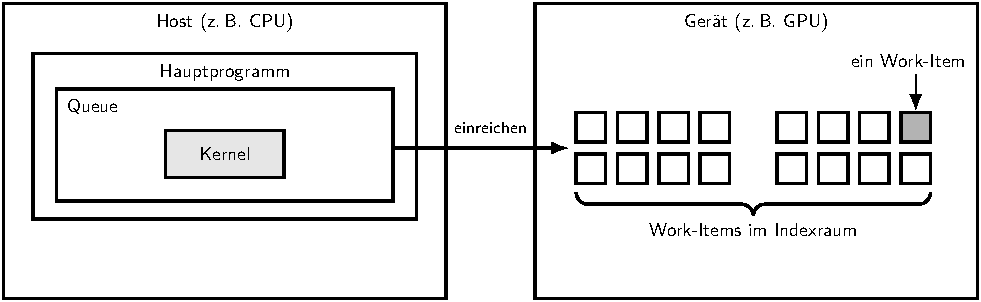
\includegraphics[width=\textwidth]{Diagramme/selbsterstellt/Stufe1.pdf}
\caption[Rollenverteilung zwischen Host und Ger\"at]{Grundaufbau eines SYCL-Programms. Der Host reicht einen Kernel \"uber eine Queue ein, das Ger\"at f\"uhrt ihn als viele Work-Items in einem Indexraum aus}
\label{fig:stufe1}
\end{figure}

Die parallele Arbeit wird als Kernel beschrieben, der auf dem Gerät
vielfach gleichzeitig ausgeführt wird. Jede Instanz heißt Work-Item und
besitzt eine eindeutige Position in einem ein- bis dreidimensionalen
Indexraum. Nach dem SPMD-Prinzip (Single Program, Multiple Data)
beschreibt der Kernel das Verhalten eines einzelnen Work-Items, das über seine
Position selbst bestimmt, welche Daten es bearbeitet. Aufträge gelangen nicht
direkt an die Hardware, sondern über eine Queue, die an einen Kontext und
ein Gerät gebunden ist. Das Einreichen kehrt sofort zurück, die Ausführung
erfolgt asynchron \cite{khronos2020sycl}.

SYCL folgt dem Single-Source-Prinzip. Host- und Geräteteil eines Programms
werden gemeinsam in Standard-C++ beschrieben. Weil Beschleuniger keine
vollständigen Betriebssystemdienste bieten, ist der Sprachumfang auf dem Gerät
eingeschränkt, etwa ohne dynamische Speicherverwaltung, Ausnahmen oder Rekursion.
Der Compiler legt den Geräteteil als Zwischendarstellung (SPIR-V, PTX, LLVM-IR)
neben dem Hostprogramm ab \cite{alpay2023sscp}. Beim ersten Start übersetzt ihn
der Treiber just in time (JIT) für das konkrete Gerät. Wird stattdessen
vorab Maschinencode erzeugt (Ahead-of-Time, AOT), entfällt diese
Startlatenz auf Kosten der Portabilität zwischen Hardwaregenerationen
\cite{reinders2023dpcpp}.

\subsection{Speichermodell und Speicherhierarchie}\label{sec:k-speicher}

Da Host und Gerät getrennte Speicher besitzen können, regelt SYCL sowohl den
Datenaustausch zwischen beiden Seiten als auch die Speicherhierarchie auf dem
Gerät (Abbildungen~\ref{fig:usm} und~\ref{fig:speicherebenen}). Für den
Austausch stehen zwei Modelle bereit, Unified Shared Memory (USM) sowie Buffer
mit Accessoren \cite{khronos2020sycl}.

\begin{figure}[htbp]
\centering
% Quelle: Diagramme/selbsterstellt/draw.drawio
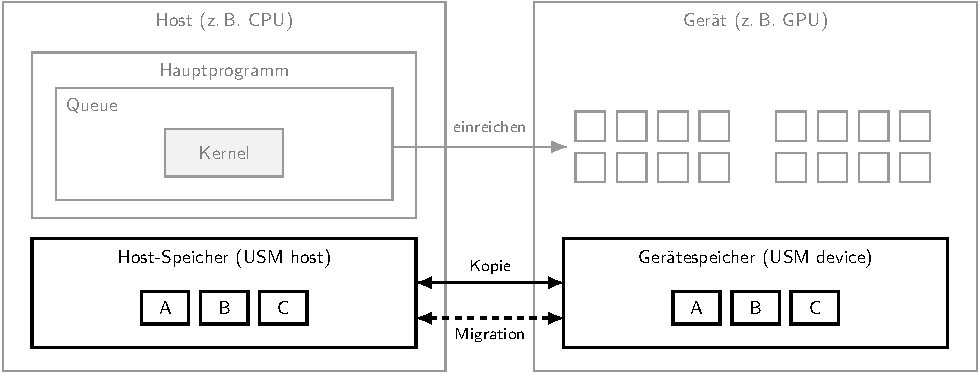
\includegraphics[width=\textwidth]{Diagramme/selbsterstellt/Speicher.pdf}
\caption[Speichermodell zwischen Host und Ger\"at]{Speichermodell, aufbauend auf Abbildung~\ref{fig:stufe1}. Neu sind Host- und Ger\"atespeicher mit den Matrizen $A$, $B$ und $C$. Bei USM device kopiert der Host die Daten ausdr\"ucklich, bei gemeinsamem Speicher verschiebt die Laufzeit sie automatisch}
\label{fig:usm}
\end{figure}

USM behält die gewohnte Arbeit mit Speicheradressen bei und unterscheidet drei
Arten von Speicher. Gerätespeicher liegt ausschließlich auf dem Gerät und
muss ausdrücklich hin- und zurückkopiert werden. Host-Speicher liegt auf
dem Host, das Gerät greift über den Systembus direkt darauf zu.
Gemeinsamer Speicher ist von beiden Seiten aus erreichbar, die Laufzeit
verschiebt die Daten bei Bedarf automatisch. Das erleichtert die Portierung,
nimmt dem Programm aber die Kontrolle über Zeitpunkt und Umfang der Transfers.

Buffer und Accessoren trennen dagegen Datenhaltung und Zugriff
\cite{reinders2023dpcpp}. Ein Buffer verwaltet Daten unabhängig davon, wo sie
gerade physisch liegen, und über einen Accessor gibt jeder Auftrag an, ob er liest,
schreibt oder beides. Daraus leitet die Laufzeit alle Kopien selbst ab und
schreibt geänderte Daten automatisch zurück, sobald der Buffer nicht mehr
benötigt wird.

Auf dem Gerät unterscheidet SYCL drei Speicherebenen
(Abbildung~\ref{fig:speicherebenen}) \cite{hwu2022pmpp}. Der
globale Speicher ist für alle Work-Items sichtbar und am größten, aber
langsam. Der lokale Speicher ist ein kleiner, schneller Speicher auf dem
Chip (auf GPUs etwa Shared Memory), den sich die Work-Items einer Work-Group
teilen. Der private Speicher gehört einem einzelnen Work-Item und liegt
bevorzugt in Registern. Mehrfach benötigte Daten aus dem globalen in den lokalen
oder privaten Speicher zu verlagern, ist der zentrale Hebel für Bandbreite und
Rechenleistung.

\begin{figure}[htbp]
\centering
% Quelle: Diagramme/selbsterstellt/draw.drawio
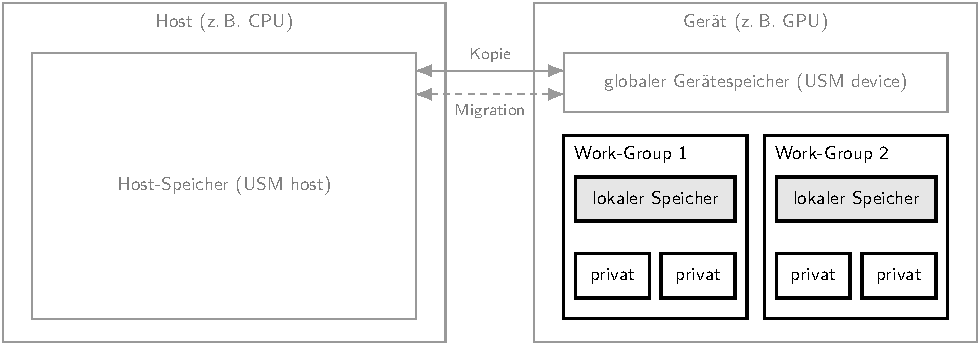
\includegraphics[width=\textwidth]{Diagramme/selbsterstellt/Speicherebenen.pdf}
\caption[Speicherebenen auf dem Ger\"at]{Speicherebenen in SYCL, aufbauend auf Abbildung~\ref{fig:usm}. Neu sind die ger\"ateinternen Ebenen je Work-Group (lokaler Speicher) und je Work-Item (privat), die nach unten kleiner und schneller werden}
\label{fig:speicherebenen}
\end{figure}

\subsection{Asynchrone Ausführung und Abhängigkeitsgraph}\label{sec:k-abhaengigkeiten}

Weil Kernel und Speichertransfers asynchron eingereicht werden, braucht die
Laufzeit eine Ordnung, die Race Conditions verhindert. Grundeinheit ist die
Command Group. Sie bündelt genau eine Aktion, etwa einen Kernel oder
einen Transfer, mit ihren Vorbedingungen und liefert sofort ein Event
zurück, das den Auftrag repräsentiert \cite{khronos2020sycl}.

Eine SYCL-Queue arbeitet standardmäßig out-of-order. Unabhängige Aufträge
dürfen in beliebiger Reihenfolge und überlappend ausgeführt werden, sodass etwa
Datentransfers parallel zu einem laufenden Kernel stattfinden können
(Abbildung~\ref{fig:dag}, links). Eine In-Order-Queue bildet dagegen eine
lineare Kette, in der jeder Auftrag erst nach Abschluss des Vorgängers startet
(rechts). Das vereinfacht streng sequentielle Zeitschrittverfahren, schließt aber
Nebenläufigkeit zwischen unabhängigen Zweigen aus \cite{reinders2023dpcpp}.

\begin{figure}[htbp]
\centering
\begin{tikzpicture}[font=\scriptsize]
    % Links: Out-of-Order DAG
    \draw[neu] (0,0) rectangle (9.8,2.75);
    \node[anchor=north, titel] at (4.9,2.70) {Out-of-Order-Queue mit gerichtetem Abhängigkeitsgraph (DAG)};
    \node[auftrag, neu, minimum width=1.85cm] (t1) at (1.20,1.98) {Transfer $D_1$};
    \node[auftrag, neu, minimum width=1.85cm] (t2) at (1.20,1.30) {Transfer $D_2$};
    \node[auftrag, neu, minimum width=1.85cm] (t3) at (1.20,0.62) {Transfer $D_3$};
    \node[auftrag, kastengrau, neu, minimum width=1.75cm] (k1) at (3.72,1.64) {Kernel $K_1$};
    \node[auftrag, kastengrau, neu, minimum width=1.75cm] (k2) at (6.15,1.12) {Kernel $K_2$};
    \node[auftrag, neu, minimum width=1.85cm] (rx) at (8.58,1.12) {Rücktransfer};
    \draw[->, neu] (t1.east) -- (k1.west);
    \draw[->, neu] (t2.east) -- (k1.west);
    \draw[->, neu] (k1.east) -- (k2.west);
    \draw[->, neu] (t3.east) -- (k2.west);
    \draw[->, neu] (k2.east) -- (rx.west);
    \node[anchor=south, font=\tiny, text=black!65] at (4.9,0.04)
        {Kanten explizit über Events (USM) oder implizit aus den Zugriffsarten der Accessoren (Buffer)};

    % Rechts: In-Order-Queue
    \draw[alt] (10.2,0) rectangle (14.8,2.75);
    \node[anchor=north, titel, text=black!65] at (12.5,2.70) {In-Order-Queue};
    \node[auftrag, alt, minimum width=3.7cm] (s1) at (12.5,2.04) {1.\ Transfers $D_1, D_2, D_3$};
    \node[auftrag, kastengrau, alt, minimum width=3.7cm] (s2) at (12.5,1.48) {2.\ Kernel $K_1$};
    \node[auftrag, kastengrau, alt, minimum width=3.7cm] (s3) at (12.5,0.92) {3.\ Kernel $K_2$};
    \node[auftrag, alt, minimum width=3.7cm] (s4) at (12.5,0.36) {4.\ Rücktransfer};
    \draw[->, black!45] (s1) -- (s2);
    \draw[->, black!45] (s2) -- (s3);
    \draw[->, black!45] (s3) -- (s4);
\end{tikzpicture}
\caption[Abhängigkeitsgraph (DAG) im Vergleich zur In-Order-Queue]{Nebenläufiger Abhängigkeitsgraph (DAG) einer Out-of-Order-Queue (links) gegenüber der streng linearen Abarbeitung einer In-Order-Queue (rechts)}
\label{fig:dag}
\end{figure}

In einer Out-of-Order-Queue baut die Laufzeit aus den Vorbedingungen einen
gerichteten azyklischen Graphen (DAG) auf. Bei USM gibt das Programm die
Abhängigkeiten ausdrücklich über die Events vorangegangener Aufträge an, bei
Buffern leitet die Laufzeit sie selbst aus den Lese- und Schreibzugriffen ab. Mit
dem Host synchronisiert der Graph erst, wenn das Hauptprogramm gezielt auf ein
Event, auf die gesamte Queue oder auf die Daten eines Buffers wartet.

\subsection{Hierarchische Ausführung, Barrieren und Kollektive}\label{sec:k-hierarchie}

Ein einfacher Indexraum überlässt die Einteilung in Gruppen der Laufzeit und
erlaubt weder gemeinsamen lokalen Speicher noch Synchronisation zwischen
Work-Items. Für hardwarenahe Optimierungen teilt der hierarchische Indexraum
(ND-Range) den globalen Bereich in Work-Groups fester Größe, die
sich weiter in Sub-Groups gliedern (Abbildung~\ref{fig:hierarchie},
links) \cite{khronos2020sycl}. Jedes Work-Item kennt dann seine globale und
lokale Position sowie seine Gruppe. Diese Hierarchie lässt sich auf GPUs (Grid,
Thread-Block, Warp bzw.\ Wavefront, Hardware-Thread) ebenso abbilden wie auf CPUs
(alle Kerne, Betriebssystem-Thread, SIMD-Vektor, SIMD-Lane) (rechts).

\begin{figure}[htbp]
\centering
\begin{tikzpicture}[font=\scriptsize]
    % Links: ND-Range Gitter 8x8 mit Work-Group, Sub-Group, Work-Item
    \fill[black!6] (1.65,0.45) rectangle (2.93,1.73);
    \fill[black!16] (1.65,1.09) rectangle (2.93,1.41);
    \fill[black!45] (2.29,1.09) rectangle (2.61,1.41);
    % Gitter an der Rahmenecke ausrichten (grid rastert sonst am Ursprung)
    \draw[black!35, shift={(0.37,0.45)}] (0,0) grid[step=0.32] (2.56,2.56);
    \draw[line width=0.7pt] (0.37,0.45) rectangle (2.93,3.01);
    \draw[line width=0.7pt] (1.65,0.45) -- (1.65,3.01);
    \draw[line width=0.7pt] (0.37,1.73) -- (2.93,1.73);
    \node[anchor=north, font=\scriptsize] at (1.65,0.40) {ND-Range (global / lokal)};

    \node[anchor=west] (lwg) at (3.25,2.38) {Work-Group};
    \draw[->] (lwg.west) -- (2.65,2.38);
    \node[anchor=west] (lsg) at (3.25,1.62) {Sub-Group};
    \draw[->] (lsg.west) -- (2.80,1.28);
    \node[anchor=west] (lwi) at (3.25,0.88) {Work-Item};
    \draw[->] (lwi.west) -- (2.50,1.20);

    % Rechts: Hardware-Abbildung (Klammern schützen Schrägstriche in foreach!)
    \node[titel] at (7.65,2.90) {SYCL-Ebene};
    \node[titel] at (10.50,2.90) {GPU-Abbildung};
    \node[titel] at (13.45,2.90) {CPU-Abbildung};

    \foreach \y/\s/\g/\c in {
        2.32/{ND-Range}/{Grid (gesamte GPU)}/{alle CPU-Kerne},
        1.72/{Work-Group}/{Thread-Block (SM)}/{OS-Thread / Kern},
        1.12/{Sub-Group}/{Warp / Wavefront}/{SIMD-Vektor},
        0.52/{Work-Item}/{Hardware-Thread}/{SIMD-Lane}%
    } {
        \node[kastengrau, neu, minimum width=2.10cm, minimum height=0.42cm] (sa) at (7.65,\y) {\s};
        \node[kasten, minimum width=2.50cm, minimum height=0.42cm] (ga) at (10.50,\y) {\g};
        \node[kasten, minimum width=2.50cm, minimum height=0.42cm] (ca) at (13.45,\y) {\c};
        \draw[-] (sa.east) -- (ga.west);
        \draw[-] (ga.east) -- (ca.west);
    }
\end{tikzpicture}
\caption[Hierarchischer Indexraum und Hardware-Abbildung]{Zerlegung einer ND-Range in Work-Groups, Sub-Groups und Work-Items (links) sowie deren Abbildung auf GPU- und CPU-Architekturen (rechts)}
\label{fig:hierarchie}
\end{figure}

Alle Work-Items einer Work-Group laufen auf derselben Recheneinheit und teilen
sich deren lokalen Speicher. Da die Reihenfolge, in der sie ausgeführt werden,
nicht festgelegt ist, trennt eine Barriere gemeinsame Lade- und
Lesephasen. Sie hält alle Work-Items der Gruppe an, bis jedes sie erreicht hat,
und macht deren Schreibzugriffe füreinander sichtbar. Zwischen verschiedenen
Work-Groups synchronisiert erst das Ende des Kernels \cite{hwu2022pmpp}.

Ergänzend bietet SYCL~2020 Gruppenkollektive wie Reduktion, Präfixsumme
oder das Verteilen eines Werts an alle Work-Items einer Gruppe, die der Compiler
auf schnelle Registeraustauschbefehle (etwa Warp-Shuffles) abbilden kann, ohne
Umweg über den lokalen Speicher. Für Reduktionen über den gesamten Indexraum
stellt SYCL eine fertige Reduktionsabstraktion bereit, die die mehrstufige
Zusammenführung übernimmt. Müssen Werte dennoch gleichzeitig aus mehreren
Gruppen aktualisiert werden, sorgen atomare Operationen für korrekte
Ergebnisse. Ihre Speicherordnung und ihr Sichtbarkeitsbereich (Gruppe oder
ganzes Gerät) lassen sich gezielt eingrenzen \cite{khronos2020sycl}.

\subsection{Laufzeitanpassung, Spezialisierung und Fehlerbehandlung}\label{sec:k-anpassung}

Da sich gute Werte für Gruppen- oder Kachelgrößen zwischen Architekturen
unterscheiden und Hardwaregrenzen nicht überschritten werden dürfen, ergänzt
SYCL das Modell um drei Laufzeitmechanismen
(Abbildung~\ref{fig:laufzeitanpassung}).

\begin{figure}[htbp]
\centering
\begin{tikzpicture}[font=\scriptsize]
    % Beteiligte und ihre Lebenslinien
    \node[kastengrau, neu, minimum width=2.7cm] (h) at (1.5,4.15) {Host-Programm};
    \node[kastengrau, neu, minimum width=3.1cm] (r) at (7.3,4.15) {SYCL-Laufzeit \& JIT};
    \node[kastengrau, neu, minimum width=2.7cm] (d) at (13.1,4.15) {Zielgerät};
    \draw[black!45] (1.5,3.92) -- (1.5,0.00);
    \draw[black!45] (7.3,3.92) -- (7.3,0.00);
    \draw[black!45] (13.1,3.92) -- (13.1,0.00);

    % 1. Geraeteabfrage
    \draw[->, neu] (1.5,3.50) -- node[above] {1.\ Geräteabfrage (Grenzen)} (7.3,3.50);
    \draw[->, dashed] (7.3,3.00) -- node[above] {Hardwareparameter des Geräts} (1.5,3.00);

    % 2. Einreichen, Uebersetzung, synchroner Fehler
    \draw[->, neu] (1.5,2.50) -- node[above] {2.\ Einreichen und Spezialisierung} (7.3,2.50);
    \draw[->, neu] (7.3,2.00) -- node[above] {JIT-Übersetzung und Start} (13.1,2.00);
    \draw[->, neu] (7.3,1.50) -- node[above] {synchron, sofortige Ausnahme} (1.5,1.50);

    % 3. Asynchrone Fehlerbehandlung
    \node[kasten, minimum width=2.5cm] (err) at (13.1,1.00) {Laufzeitfehler am Gerät};
    \draw[->, dashed] (err.west) -- node[above] {gesammelt} (7.3,1.00);
    \draw[->, neu] (1.5,0.50) -- node[above] {3.\ Warten und Fehler abholen} (7.3,0.50);
    \draw[->, neu] (7.3,0.00) -- node[above] {asynchron, Fehlerbehandler} (1.5,0.00);
\end{tikzpicture}
\caption[Laufzeitanpassung, Spezialisierung und zweigeteilte Fehlerbehandlung]{Zusammenspiel von Geräteabfragen, JIT-Spezialisierung sowie synchroner und asynchroner Fehlerbehandlung}
\label{fig:laufzeitanpassung}
\end{figure}

\begin{itemize}[nosep]
    \item Geräteabfragen. Vor dem Start eines Kernels kann der Host
    Eigenschaften des Geräts abfragen, etwa die Zahl der Recheneinheiten, die
    maximale Work-Group-Größe sowie die Größe von lokalem und globalem Speicher
    \cite{khronos2020sycl}. So lassen sich ungültige Konfigurationen ausschließen
    und Parameter passend zum Gerät wählen.
    \item Specialization Constants. Werte, die erst zur Laufzeit
    feststehen, werden vor der JIT-Übersetzung als Konstanten in den Kernel
    eingesetzt. Der Compiler kann sie dann wie feste Werte behandeln und etwa
    Schleifen abrollen. SPIR-V unterstützt dies direkt, während PTX-Backends es
    über einen Hilfsspeicher nachbilden \cite{dpcpp_spec_const} oder
    Erweiterungen benötigen \cite{adaptivecpp_ext}.
    \item Fehlerbehandlung. Synchrone Fehler, die schon beim
    Einreichen erkannt werden (etwa eine unzulässige Gruppengröße), meldet SYCL
    sofort als Ausnahme im Hostprogramm \cite{reinders2023dpcpp}.
    Asynchrone Fehler, die erst bei der Ausführung auf dem Gerät
    auftreten, sammelt die Laufzeit und übergibt sie an einen Fehlerbehandler der
    Queue, sobald der Host auf deren Abschluss wartet.
\end{itemize}

\newpage
% ---------------------------------------------------------------------------
\section{Ergebnisse}\label{sec:ergebnisse}

Sämtliche Stufen und Varianten liefen ohne Codeänderung auf allen vier
Zielgeräten und lieferten korrekte Ergebnisse. Abbildung~\ref{fig:cuda_vergleich}
vergleicht sie mit denselben Programmen in CUDA, der herstellereigenen Sprache
für NVIDIA-GPUs, die Einzelwerte stehen in Anhang~\ref{sec:messungen}.

\begin{figure}[htbp]
\centering
\pgfplotsset{
    every axis/.append style={
        font=\scriptsize,
        line width=0.4pt,
        grid style={black!20, densely dotted}, ymajorgrids,
        tick align=outside, tick pos=left,
        legend style={draw=none, fill=none, font=\scriptsize},
        legend cell align=left,
    }
}
\begin{tikzpicture}
\begin{axis}[
    width=13.5cm, height=4.2cm, ybar, bar width=6pt, enlarge x limits=0.11,
    ymin=0, ymax=180, ytick={0,50,100,150},
    symbolic x coords={m3,m4,s2d,slok,rbaum,rbuilt}, xtick=data,
    xticklabels={
        {Matmul\\global (St.\,3)},
        {Matmul\\Kachel ($T{=}16$)},
        {Stencil\\2D global},
        {Stencil\\lokal ($T{=}16$)},
        {Reduktion\\Baum lokal},
        {Reduktion\\eingebaut (CUB)}
    },
    xticklabel style={align=center, font=\scriptsize},
    ylabel={Relative Leistung (\% von CUDA / CUB)},
    legend style={at={(0.5,1.02)}, anchor=south, legend columns=3, /tikz/every even column/.append style={column sep=10pt}},
    legend image code/.code={\draw[#1] (0cm,-0.08cm) rectangle (0.3cm,0.1cm);},
]
\addplot[fill=black!45, draw=black, line width=0.4pt]
    coordinates {(m3,104) (m4,69) (s2d,97) (slok,101) (rbaum,96) (rbuilt,85)};
\addlegendentry{RTX 5060 Ti}
\addplot[fill=black!75, draw=black, line width=0.4pt]
    coordinates {(m3,108) (m4,72) (s2d,100) (slok,98) (rbaum,28) (rbuilt,77)};
\addlegendentry{L40S}
\addplot[fill=black!15, draw=black, line width=0.4pt]
    coordinates {(m3,100) (m4,80) (s2d,81) (slok,162) (rbaum,5) (rbuilt,37)};
\addlegendentry{H100}
\draw[dashed, black!60, line width=0.5pt] ({rel axis cs:0,0}|-{axis cs:m3,100}) -- ({rel axis cs:1,0}|-{axis cs:m3,100});
\end{axis}
\end{tikzpicture}
\caption[SYCL im Vergleich zu nativem CUDA über alle Fallbeispiele]{Leistung relativ zu nativem CUDA bzw.\ CUB bei der jeweils größten Problemgröße ($n=2048$, $n=8192$ bzw.\ $n=2^{26}$), gestrichelt 100\,\%}
\label{fig:cuda_vergleich}
\end{figure}

\subsection{Matrixmultiplikation}\label{sec:e-matmul}

\paragraph{Grundparallelisierung und Speichermodell.}
Den größten Sprung bringt die Parallelisierung selbst (Stufe~1). Bei $n = 1024$
rechnet sie 87-mal schneller als das sequentielle Programm auf einem CPU-Kern,
auf der H100 15\,600-mal (Tabelle~\ref{tab:stufenmessung}). Eigener
Gerätespeicher (Stufe~2) ändert die Rechenzeit nicht ($\le 0{,}4\,\%$), macht
aber das Kopieren zwischen Rechner und Gerät sichtbar, das auf der H100 auf
74\,\% der Rechenzeit anwächst (Tabelle~\ref{tab:zeiten}). Je Lauf neu angelegte Buffer (Stufe~2b) kosten 12 bis 64\,\% Gesamtzeit.

\paragraph{Gruppen, Kachelung und Kachelgröße.}
Teilt das Programm die Arbeit selbst in Gruppen ein (Stufe~3), steigt der
Durchsatz um 19 bis 89\,\%. Mit Kacheln im schnellen Speicher der Gruppe
(Stufe~4) sind es 28 bis 68\,\% und auf der CPU das 3,5-Fache, auf RTX und L40S
aber 11\,\% weniger als mit Stufe~3.

Die beste Kachelgröße hängt vom Gerät ab (Abbildung~\ref{fig:ergebnisse},
Tabelle~\ref{tab:kacheln}). Auf allen GPUs sind $16 \times 16$ Felder optimal,
auf der CPU $32 \times 32$ bzw.\ $64 \times 64$. Eine 64er-Kachel braucht 4096
Work-Items je Gruppe und überschreitet die GPU-Grenze von 1024, dort startet das
Programm gar nicht (Portabilitätswert~0). Stufe~5 fragt die Grenze ab und
vermeidet den Ausfall. Auf der CPU erreicht sie mit 179\,GFLOPS den
besten Wert, auf den GPUs trotz gleicher Kachel 5 bis 43\,\% weniger als
Stufe~4, weil DPC++ die erst beim Start gewählte Größe nachbilden muss
\cite{dpcpp_spec_const}.

\paragraph{Abstand zu nativem CUDA.}
In Stufe~3 liegt SYCL gleichauf (100 bis 108\,\%), fällt in Stufe~4 auf 69 bis
80\,\% zurück (Tabelle~\ref{tab:matmul_cuda}), weil DPC++ den schnellen
Gruppenspeicher schlechter übersetzt. Von der Herstellerbibliothek cuBLAS
\cite{nvidia_cublas} sind beide um den Faktor~5 bis~7 entfernt, weil sie
Zwischenwerte nicht in Registern halten \cite{volkov2008gemm}.

\subsection{Stencil}\label{sec:e-stencil}

\paragraph{Speichermodell.}
Stufe~2 erreicht 81 bis 100\,\% des CUDA-Programms
(Tabellen~\ref{tab:stencil} und~\ref{tab:stencil_stufen}). Der Stencil rechnet
kaum, deshalb verdeckt keine Rechenzeit die Kosten des Speichermodells.
Automatisch verschobener Speicher
kostet bis zu 74\,\% Bandbreite, ein je Lauf neu angelegter Buffer bis zu
60\,\% und ein wiederverwendeter noch 23 bis 43\,\%.

\paragraph{Gruppengröße und lokaler Speicher.}
Den größten Gewinn bringt die selbst gewählte Gruppengröße. Mit 16 Work-Items je
Gruppe erreicht die H100 101\,\% statt 81\,\%, der Rückstand entstand also
allein aus der Gruppeneinteilung der Laufzeit. Kacheln samt Rand (Stufe~4)
lohnen kaum, weil die Zwischenspeicher der Hardware dasselbe leisten. Auf der H100 schaden sie CUDA ($-60\,\%$) stärker als SYCL
($-20\,\%$), das dort 62\,\% schneller ist.

\paragraph{Laufzeitanpassung und Indexraum.}
Stufe~5 kostet durch dasselbe Nachbilden je Kernelstart 12\,\% (L40S) bzw.\
54\,\% (H100). Nummeriert man das Gitter eindimensional statt zweidimensional,
kostet das entgegen Abram et al.\ \cite{abram2025sycl} auf allen Geräten 25 bis
73\,\% Bandbreite.

\subsection{Reduktion}\label{sec:e-reduktion}

\paragraph{Speichermodell und Atomics.}
Addieren alle Work-Items ihren Wert unmittelbar auf dasselbe Ergebnis (Stufe~2),
braucht SYCL das 6300- bis 20\,500-Fache der CUDA-Zeit
(Tabellen~\ref{tab:reduktion} und~\ref{tab:reduktion_stufen}). DPC++ nutzt dafür
nicht den Hardwarebefehl, sondern eine Schleife, die jeden Versuch wiederholt,
bis kein anderes Work-Item dazwischenkommt. Anders als beim
Stencil überdeckt das jeden Unterschied zwischen den Speichermodellen
($\le 0{,}6\,\%$).

\paragraph{Gruppengröße und lokaler Speicher.}
Den größten Gewinn bringt es, zuerst innerhalb jeder Gruppe paarweise zu
summieren (Stufen~3/4). Das senkt die Zugriffe auf das Gesamtergebnis von rund
einer Million auf 4096 und erreicht auf der RTX 96\,\%, je mehr Recheneinheiten
ein Gerät hat aber nur noch 28\,\% (L40S) und 5\,\% (H100).

\paragraph{Laufzeitanpassung und Abstraktion.}
Stufe~5 bildet über Geräteabfragen nur noch rund 1100 Gruppen und erreicht auf
der L40S 99\,\% der NVIDIA-Bibliothek CUB \cite{nvidia_cub}, auf der H100 nur
21\,\%. Dort schlägt die fertige Reduktion von SYCL mit 37\,\% alle eigenen
Stufen, sonst bleibt sie dahinter.

\newpage
% ---------------------------------------------------------------------------
\section{Diskussion}\label{sec:diskussion}
% ---------------------------------------------------------------------------

\paragraph{F1 -- Konzepte und Problemlösung.}
Herstellerbindung und doppelte Codebasen überwindet SYCL schon auf der untersten
Stufe. Weil Host- und Geräteteil in derselben C++-Datei stehen, läuft derselbe
Quellcode, auf einem Rechner sogar dieselbe ausführbare Datei, unverändert auf
CPU und GPU\@. Den Zielkonflikt zwischen Abstraktion und Kontrolle löst das
Programmiermodell dadurch, dass sich seine Konzepte einzeln zuschalten lassen.
Für eine erste, korrekte Portierung genügen ein flacher Indexraum und
automatisch verschobener Speicher. Wer mehr Leistung braucht, übernimmt Kopien,
Gruppeneinteilung und lokalen Speicher selbst. Bequemlichkeit kostet dabei
messbar, bei speichergebundenen Programmen 23 bis 74\,\% Bandbreite.

\paragraph{F2 -- Performance-Portabilität.}
Funktionale Portabilität ist über alle Stufen gegeben, gleich gute Leistung
stellt sich jedoch nicht von selbst ein. Zum einen bleiben Kachel- und
Gruppengröße an die Hardware gebunden. Die auf der CPU beste Kachelgröße
überschreitet die Grenze aller GPUs, dort startet das Programm gar nicht, und
beim Stencil entscheidet allein die Gruppengröße zwischen 81 und 101\,\% der
CUDA-Leistung. Geräteabfragen in Stufe~5 verhindern solche Abbrüche und finden
überall brauchbare Werte, die Auswahl der Stellschrauben nehmen sie dem
Entwickler aber nicht ab. Zum anderen hängt der Abstand zu CUDA davon ab, wie gut
die Implementierung für das Zielgerät übersetzt \cite{deakin2020sycl}. Einfache
Programme erreichen 81 bis 108\,\%, während nachgebildete statt direkt
umgesetzte Sprachmittel -- vor allem atomare Gleitkommaoperationen -- bis auf
5\,\% einbrechen. Welche Stufe sich lohnt, hängt zudem vom Problem ab, bei
rechengebundener Last die Kachelung, bei speichergebundener das Speichermodell
und die Vermeidung atomarer Engpässe.

\paragraph{Methodische Grenzen.}
Untersucht wurden drei einfach gebaute Programme mit einer einzigen
SYCL-Implementierung und GPUs nur eines Herstellers, da die AMD-Karte im
Messzeitraum nicht verfügbar war. Die Portabilitätszahl misst nur den Abstand zur
besten eigenen Variante auf genau diesen Geräten
\cite{pennycook2019implications}, während die Herstellerbibliothek auch die
handgeschriebenen CUDA-Programme um das 5- bis 7-Fache schlägt. SYCL wurde ohne
Festlegung auf eine GPU übersetzt, CUDA dagegen gerätespezifisch, und je
Messpunkt nur der Median aus fünf Läufen gebildet.

\paragraph{Fazit und Ausblick.}
SYCL löst das Versprechen \enquote{ein Quellcode für heterogene Hardware}
funktional vollständig ein und bietet ein Modell, das sich schrittweise
vertiefen lässt. Hohe Leistung verlangt aber weiterhin, Parameter bewusst an die
Architektur anzupassen und eine Implementierung zu wählen, die für das Zielgerät
guten Code erzeugt. Künftige Arbeiten sollten AMD- und Intel-GPUs sowie
AdaptiveCpp einbeziehen und prüfen, wie viel eine gerätespezifische Übersetzung
an diesen Schwachstellen ändert.

\newpage
\markboth{Literaturverzeichnis}{}
\printbibliography[heading=bibintoc, title={Literaturverzeichnis}]

% ---------------------------------------------------------------------------
% Anhang
% ---------------------------------------------------------------------------
\newpage
\appendix
\section{Messergebnisse}\label{sec:messungen}

\subsection{Messbedingungen}\label{sec:messbedingungen}

\begin{itemize}[nosep]
    \sloppy
    \item SYCL. DPC++~7.2 (Open-Source-Release von
    \texttt{intel/\allowbreak llvm}), kompiliert mit \texttt{-fsycl} \texttt{-O3} und
    \texttt{-fsycl-targets=\allowbreak nvptx64-\allowbreak nvidia-\allowbreak cuda,\allowbreak spir64}
    ohne explizites \texttt{-{}-cuda-\allowbreak gpu-\allowbreak arch}. Das Zielgerät wird zur Laufzeit
    über \texttt{ONEAPI\_\allowbreak DEVICE\_\allowbreak SELECTOR} gewählt, GPUs über das CUDA-Backend und
    der Ryzen~5~5600X über die Intel OpenCL-CPU-Laufzeit. Das sequentielle
    Ausgangsprogramm (Stufe~0) wird mit \texttt{g++ -O3 -std=c++17} übersetzt.
    \item Hardware. Arbeitsplatzrechner mit AMD Ryzen~5~5600X (6 Kerne)
    und NVIDIA GeForce RTX~5060~Ti (16\,GB, CUDA~13.4) sowie DACHS-Cluster der
    Hochschule Esslingen mit L40S (Host AMD EPYC~9254) und
    H100 80\,GB HBM3 (Host AMD EPYC~9454), jeweils CUDA-Toolkit~12.8 auf
    Treiber-CUDA~13.2.
    \item CUDA. Übersetzt mit \texttt{nvcc -O3 -std=c++17} und
    \texttt{-arch=native} (RTX) bzw.\ auf DACHS mit \texttt{-gencode} für
    \texttt{compute\_89}/\texttt{sm\_89} (L40S) und
    \texttt{compute\_90}/\texttt{sm\_90} (H100).
    Der Kernel im globalen Speicher nutzt feste $16 \times 16$-Blöcke
    und entspricht damit Stufe~3 mit $W = 16$, da CUDA stets eine Blockgröße
    verlangt. Der gekachelte Kernel im Shared Memory entspricht Stufe~4 für
    $T \in \{8, 16, 32, 64\}$.
    \item cuBLAS. SGEMM in einfacher Genauigkeit (FP32). Die
    TF32-Tensor-Cores sind abgeschaltet
    (\texttt{CUBLAS\_\allowbreak PEDANTIC\_\allowbreak MATH}), damit dieselbe
    Rechengenauigkeit verglichen wird wie in den eigenen Kerneln.
    \item Problemgrößen. Matrixmultiplikation $n = 1024$ und $n = 2048$
    (Stufe~0 nur bis $n = 1024$). Stencil $n = 8192$ (256\,MB je Gitter) mit
    100 Zeitschritten. Reduktion $n = 2^{26}$ (256\,MB). Kleinere Probleme
    ($n = 2^{24}$, 64\,MB) passen in den L2-Cache der L40S (96\,MB) und messen
    deshalb den Cache statt des Speichers, sie sind nicht dargestellt.
    \item Zeitmessung. \texttt{std::chrono::steady\_clock} auf dem Host,
    Median aus fünf Läufen nach einem getrennt erfassten ersten Lauf. Zwei
    unabhängige Messläufe von Stencil und Reduktion auf der H100 zeigten
    Abweichungen $\le 1\,\%$ (Stencil) bzw.\ $\le 4\,\%$ (Reduktion). Das
    Kachelgrößen-Experiment (Tabelle~\ref{tab:kacheln}) wurde in einem eigenen
    Durchlauf erfasst, ebenso die Stufenvergleiche von Stencil und Reduktion
    (Tabellen~\ref{tab:stencil_stufen} und~\ref{tab:reduktion_stufen}) am
    19.11.2026 auf L40S und H100.
\end{itemize}

\subsection{Matrixmultiplikation}\label{sec:a-matmul}

\begin{table}[H]
\centering
\footnotesize
\setlength{\tabcolsep}{4pt}
\caption[Leistung je Stufe bei der Matrixmultiplikation (GFLOPS)]{Leistung je Stufe der Matrixmultiplikation in GFLOPS für $n = 1024$ und $n = 2048$ (Median aus fünf Läufen). Stufe~0 läuft auf einem Kern der jeweiligen Host-CPU (Ryzen~5~5600X bzw.\ EPYC~9254 / 9454)}
\label{tab:stufenmessung}
\begin{tabular}{@{}l*{8}{>{\raggedleft\arraybackslash}p{1.12cm}}@{}}
\toprule
 & \multicolumn{2}{c}{RTX 5060 Ti} & \multicolumn{2}{c}{L40S} & \multicolumn{2}{c}{H100} & \multicolumn{2}{c}{Ryzen 5 5600X} \\
\cmidrule(lr){2-3}\cmidrule(lr){4-5}\cmidrule(lr){6-7}\cmidrule(l){8-9}
Stufe & 1024 & 2048 & 1024 & 2048 & 1024 & 2048 & 1024 & 2048 \\
\midrule
0 (ein CPU-Kern)                 &    0,5 &     -- &    0,3 &     -- &    0,4 &     -- &   0,5 &     -- \\
1 (USM shared)                   & 1102,0 & 1108,0 & 3489,0 & 2938,0 & 6044,0 & 4793,0 &  43,0 &   43,0 \\
2 (USM device)                   & 1094,0 & 1110,0 & 3471,0 & 2938,0 & 6110,0 & 4811,0 &  41,0 &   43,0 \\
2b (Buffer, mit Transfer)        &  645,0 &  863,0 & 1261,0 & 1847,0 & 1246,0 & 2468,0 &  31,0 &   28,0 \\
3 (\texttt{nd\_range}, $W = 16$) & 1573,0 & 1595,0 & 5231,0 & 5563,0 & 4858,0 & 5351,0 &  51,0 &   51,0 \\
4 (Kachelung, $T = 16$)          & 1388,0 & 1426,0 & 4704,0 & 4933,0 & 5853,0 & 6348,0 & 151,0 &  149,0 \\
5 (angepasst)                    & 1240,0 & 1350,0 & 3624,0 & 4678,0 & 3317,0 & 5497,0 & 179,0 &  176,0 \\
\bottomrule
\end{tabular}
\end{table}

\begin{table}[H]
\centering
\footnotesize
\setlength{\tabcolsep}{3.5pt}
\caption[Laufzeit je Stufe bei der Matrixmultiplikation (ms)]{Laufzeit je Stufe der Matrixmultiplikation in ms für $n = 1024$ und $n = 2048$ (Median aus fünf Läufen, exemplarisch mit erstem Lauf für Stufen~1, 4 und~5). Ab Stufe~2 sind Kernel- und Transferzeit getrennt erfasst, außer bei Stufe~2b}
\label{tab:zeiten}
\begin{tabular}{@{}l*{8}{r}@{}}
\toprule
 & \multicolumn{2}{c}{RTX 5060 Ti} & \multicolumn{2}{c}{L40S} & \multicolumn{2}{c}{H100} & \multicolumn{2}{c}{Ryzen 5 5600X} \\
\cmidrule(lr){2-3}\cmidrule(lr){4-5}\cmidrule(lr){6-7}\cmidrule(l){8-9}
Stufe & 1024 & 2048 & 1024 & 2048 & 1024 & 2048 & 1024 & 2048 \\
\midrule
0 (ein CPU-Kern)              & 4319,38 & --     & 6665,88 & --    & 5600,27 & --    & 4319,38 & --      \\
1 (USM shared)                & 1,95    & 15,50  & 0,62    & 5,85  & 0,36    & 3,58  & 49,64   & 398,64  \\
\quad erster Lauf (JIT)       & 4,28    & 23,06  & 4,47    & 13,63 & 4,93    & 13,08 & 178,39  & 526,63  \\
2 Kernel                      & 1,96    & 15,47  & 0,62    & 5,85  & 0,35    & 3,57  & 52,51   & 398,78  \\
\quad Transfer                & 1,14    & 4,16   & 0,61    & 2,17  & 0,70    & 2,65  & 0,90    & 4,97    \\
2b Kernel und Transfer        & 3,33    & 19,90  & 1,70    & 9,30  & 1,72    & 6,96  & 68,40   & 611,88  \\
3 Kernel ($W = 16$)           & 1,37    & 10,77  & 0,41    & 3,09  & 0,44    & 3,21  & 42,33   & 334,61  \\
4 Kernel ($T = 16$)           & 1,55    & 12,05  & 0,46    & 3,48  & 0,37    & 2,71  & 14,24   & 115,04  \\
\quad Transfer                & 1,53    & 4,06   & 0,59    & 3,29  & 0,72    & 2,55  & 0,70    & 4,64    \\
\quad erster Lauf (JIT)       & 3,22    & 16,55  & 3,42    & 8,85  & 3,29    & 7,25  & 142,91  & 245,22  \\
5 Kernel (angepasst)          & 1,73    & 12,73  & 0,59    & 3,67  & 0,65    & 3,13  & 11,98   & 97,72   \\
\quad erster Lauf mit Auswahl & 25,97   & 181,91 & 13,35   & 58,73 & 14,32   & 54,08 & 511,65  & 2291,03 \\
\bottomrule
\end{tabular}
\end{table}

\begin{table}[H]
\centering
\footnotesize
\setlength{\tabcolsep}{4.5pt}
\caption[Effizienz je Kachelgröße und Performance-Portabilität]{Effizienz der Matrixmultiplikation in \% der besten festen Kachelgröße desselben Geräts und Performance-Portabilität (PP) für $n = 1024$ und $n = 2048$ (\textsuperscript{*}für PP auf 100\,\% gedeckelt)}
\label{tab:kacheln}
\begin{tabular}{@{}llrrrrr@{}}
\toprule
$n$ & Kachelgröße & RTX 5060 Ti & L40S & H100 & Ryzen 5 5600X & PP \\
\midrule
1024 & $T = 8$  & 86  & 85  & 70  & 44  & 0,66 \\
     & $T = 16$ & 100 & 100 & 100 & 73  & 0,92 \\
     & $T = 32$ & 95  & 90  & 92  & 100 & 0,94 \\
     & $T = 64$ & startet nicht & startet nicht & startet nicht & 92 & 0,00 \\
     & Stufe 5 (angepasst) & 88 ($T{=}16$) & 77 ($T{=}16$) & 57 ($T{=}16$) & 97 ($T{=}32$) & 0,76 \\
\midrule
2048 & $T = 8$  & 83  & 85  & 69  & 55  & 0,71 \\
     & $T = 16$ & 100 & 100 & 100 & 88  & 0,97 \\
     & $T = 32$ & 96  & 98  & 91  & 97  & 0,95 \\
     & $T = 64$ & startet nicht & startet nicht & startet nicht & 100 & 0,00 \\
     & Stufe 5 (angepasst) & 95 ($T{=}16$) & 95 ($T{=}16$) & 87 ($T{=}16$) & 106\textsuperscript{*} ($T{=}64$) & 0,94 \\
\bottomrule
\end{tabular}
\end{table}

\begin{figure}[H]
\centering
\pgfplotsset{
    every axis/.append style={
        font=\scriptsize, width=7cm, height=3.4cm, line width=0.4pt,
        grid style={black!20, densely dotted}, ymajorgrids,
        tick align=outside, tick pos=left,
        legend style={draw=none, fill=none, font=\scriptsize},
        legend cell align=left,
    }
}
\begin{tikzpicture}
\begin{axis}[
    width=8.2cm, ybar, bar width=4.5pt, enlarge x limits=0.16,
    ymin=0, ymax=115, ytick={0,25,50,75,100},
    symbolic x coords={8,16,32,64}, xtick=data,
    xticklabels={{$T{=}8$\\PP 0{,}71},{$T{=}16$\\PP 0{,}97},{$T{=}32$\\PP 0{,}95},{$T{=}64$\\PP 0}},
    xticklabel style={align=center},
    ylabel={Effizienz in \%},
    legend style={at={(0.5,1.0)}, anchor=south, legend columns=4, /tikz/every even column/.append style={column sep=6pt}},
    legend image code/.code={\draw[#1] (0cm,-0.08cm) rectangle (0.3cm,0.1cm);},
]
\addplot[fill=black!45, draw=black, line width=0.4pt]
    coordinates {(8,83) (16,100) (32,96) (64,0)};
\addlegendentry{RTX}
\addplot[fill=black!75, draw=black, line width=0.4pt]
    coordinates {(8,85) (16,100) (32,98) (64,0)};
\addlegendentry{L40S}
\addplot[fill=black!15, draw=black, line width=0.4pt]
    coordinates {(8,69) (16,100) (32,91) (64,0)};
\addlegendentry{H100}
\addplot[fill=white, draw=black, line width=0.4pt, postaction={pattern=north east lines}]
    coordinates {(8,55) (16,88) (32,97) (64,100)};
\addlegendentry{CPU}
\node[font=\scriptsize, rotate=90, anchor=west] at ([xshift=-4.5pt]axis cs:64,2) {startet nicht};
\end{axis}
\end{tikzpicture}
\caption[Effizienz und Performance-Portabilität je Kachelgröße ($n = 2048$)]{Effizienz (Application Efficiency) und Performance-Portabilität je Kachelgröße bei $n = 2048$ in Stufe~4}
\label{fig:ergebnisse}
\end{figure}

\begin{table}[H]
\centering
\footnotesize
\setlength{\tabcolsep}{4pt}
\caption[Matrixmultiplikation im Vergleich zu CUDA und cuBLAS]{Matrixmultiplikation im Vergleich zu CUDA und cuBLAS in GFLOPS bei $n = 2048$ (FP32 ohne TF32, Median aus fünf Läufen)}
\label{tab:matmul_cuda}
\begin{tabular}{@{}l*{6}{r}@{}}
\toprule
 & \multicolumn{2}{c}{RTX 5060 Ti} & \multicolumn{2}{c}{L40S} & \multicolumn{2}{c}{H100} \\
\cmidrule(lr){2-3}\cmidrule(lr){4-5}\cmidrule(l){6-7}
Variante ($n = 2048$) & SYCL & CUDA & SYCL & CUDA & SYCL & CUDA \\
\midrule
Globaler Speicher ($W = 16$, Stufe~3) & 1595 & 1536  & 5563 & 5173  & 5351 & 5353  \\
Kachelung ($T = 16$, Stufe~4)         & 1426 & 2055  & 4933 & 6883  & 6348 & 7949  \\
Kachelung ($T = 32$, Stufe~4)         & 1362 & 1932  & 4815 & 6414  & 5774 & 8538  \\
cuBLAS SGEMM (FP32)                   & --   & 14333 & --   & 35404 & --   & 46211 \\
\bottomrule
\end{tabular}
\end{table}

\subsection{Stencil}\label{sec:a-stencil}

\begin{table}[H]
\centering
\footnotesize
\setlength{\tabcolsep}{4pt}
\caption[Effektive Bandbreite beim Stencil (GB/s)]{Effektive Bandbreite beim Stencil in GB/s (256\,MB je Gitter, 100 Zeitschritte, Median aus fünf Läufen, -- = keine CUDA-Variante)}
\label{tab:stencil}
\begin{tabular}{@{}l*{7}{r}@{}}
\toprule
 & \multicolumn{2}{c}{RTX 5060 Ti} & \multicolumn{2}{c}{L40S} & \multicolumn{2}{c}{H100} & Ryzen \\
\cmidrule(lr){2-3}\cmidrule(lr){4-5}\cmidrule(lr){6-7}\cmidrule(l){8-8}
Variante ($n = 8192$) & SYCL & CUDA & SYCL & CUDA & SYCL & CUDA & SYCL \\
\midrule
2D, globaler Speicher          &  357,0 &  368,0 &  669,0 &  671,0 & 1552,0 & 1908,0 & 15,6 \\
2D, Warten nach jedem Schritt  &  357,0 &     -- &  661,0 &     -- & 1517,0 &     -- & 16,1 \\
1D linearisiert                &  224,0 &     -- &  483,0 &     -- &  425,0 &     -- & 11,7 \\
lokaler Speicher ($T = 16$)    &  300,0 &  297,0 &  682,0 &  695,0 & 1237,0 &  765,0 &  8,7 \\
\bottomrule
\end{tabular}
\end{table}

\begin{table}[H]
\centering
\footnotesize
\setlength{\tabcolsep}{4pt}
\caption[Leistung je Stufe beim Stencil (GB/s)]{Effektive Bandbreite je Stufe beim Stencil in GB/s ($n = 8192$, 100 Zeitschritte, eigener Durchlauf vom 19.11.2026, Median aus fünf Läufen). Die relativen Angaben beziehen sich auf Stufe~2 desselben Durchlaufs}
\label{tab:stencil_stufen}
\begin{tabular}{@{}llrrrr@{}}
\toprule
 & & \multicolumn{2}{c}{L40S} & \multicolumn{2}{c}{H100} \\
\cmidrule(lr){3-4}\cmidrule(l){5-6}
Variante ($n = 8192$) & Stufe & GB/s & zu St.\,2 & GB/s & zu St.\,2 \\
\midrule
Gemeinsamer Speicher                     & 1  & 306 & $-54\,\%$ & 410  & $-74\,\%$ \\
Buffer, je Lauf neu angelegt             & 2b & 421 & $-37\,\%$ & 623  & $-60\,\%$ \\
Buffer, wiederverwendet                  & 2b & 515 & $-23\,\%$ & 878  & $-43\,\%$ \\
Gerätespeicher, 2D-Indexraum             & 2  & 668 & --        & 1553 & --        \\
Gruppengröße $W = 8$                     & 3  & 670 & $\pm 0\,\%$ & 848  & $-45\,\%$ \\
Gruppengröße $W = 16$                    & 3  & 669 & $\pm 0\,\%$ & 1931 & $+24\,\%$ \\
Gruppengröße $W = 32$                    & 3  & 700 & $+5\,\%$ & 1569 & $+1\,\%$ \\
Lokaler Speicher, $B = 16$               & 4  & 682 & $+2\,\%$  & 1238 & $-20\,\%$ \\
Geräteabfrage, Halo mit Division ($B = 16$) & 5 & 592 & $-11\,\%$ & 716  & $-54\,\%$ \\
Geräteabfrage, eigene Kachel ($B = 8$ / $16$) & 5 & 587 & $-12\,\%$ & 716  & $-54\,\%$ \\
\midrule
CUDA, globaler Speicher ($B = 16$)       & --- & 671 &           & 1910 &           \\
CUDA, lokaler Speicher ($B = 16$)        & --- & 695 &           & 762  &           \\
\bottomrule
\end{tabular}
\end{table}

\subsection{Reduktion}\label{sec:a-reduktion}

\begin{table}[H]
\centering
\footnotesize
\setlength{\tabcolsep}{4pt}
\caption[Effektive Bandbreite bei der Reduktion (GB/s)]{Effektive Bandbreite bei der Reduktion in GB/s (256\,MB, Median aus fünf Läufen, -- = keine CUDA-Variante)}
\label{tab:reduktion}
\begin{tabular}{@{}l*{7}{r}@{}}
\toprule
 & \multicolumn{2}{c}{RTX 5060 Ti} & \multicolumn{2}{c}{L40S} & \multicolumn{2}{c}{H100} & Ryzen \\
\cmidrule(lr){2-3}\cmidrule(lr){4-5}\cmidrule(lr){6-7}\cmidrule(l){8-8}
Variante ($n = 2^{26}$) & SYCL & CUDA & SYCL & CUDA & SYCL & CUDA & SYCL \\
\midrule
Atomic je Work-Item                  &   0,03 &  202,00 &   0,01 &  158,00 &    0,01 &  142,00 &  2,40 \\
Baum im lokalen Speicher             & 404,00 &  419,00 & 206,00 &  738,00 &  111,00 & 2166,00 & 17,90 \\
\texttt{reduce\_over\_group}         & 406,00 &      -- & 209,00 &      -- &  106,00 &      -- & 17,10 \\
eingebaut (\texttt{reduction}/CUB)   & 356,00 &  419,00 & 551,00 &  715,00 & 1020,00 & 2792,00 & 16,00 \\
\bottomrule
\end{tabular}
\end{table}

\begin{table}[H]
\centering
\footnotesize
\setlength{\tabcolsep}{4pt}
\caption[Leistung je Stufe bei der Reduktion (GB/s)]{Effektive Bandbreite je Stufe bei der Reduktion in GB/s ($n = 2^{26}$, eigener Durchlauf vom 19.11.2026, Median aus fünf Läufen). Die letzte Spalte nennt die Zahl der atomaren Zugriffe auf das Gesamtergebnis}
\label{tab:reduktion_stufen}
\begin{tabular}{@{}llrrl@{}}
\toprule
Variante ($n = 2^{26}$) & Stufe & L40S & H100 & Atomare Zugriffe \\
\midrule
Gemeinsamer Speicher                  & 1  & 0,01 (31,1\,s) & 0,01 (38,3\,s) & $2^{20}$ \\
Gerätespeicher, Atomic je Work-Item   & 2  & 0,01 (31,0\,s) & 0,01 (38,6\,s) & $2^{20}$ \\
Buffer, je Lauf neu angelegt          & 2b & 0,01 (31,0\,s) & 0,01 (38,5\,s) & $2^{20}$ \\
Buffer, wiederverwendet               & 2b & 0,01 (31,0\,s) & 0,01 (38,5\,s) & $2^{20}$ \\
Baum im lokalen Speicher ($W = 256$)  & 3/4 & 211,00 &  111,00 & 4096 \\
\texttt{reduce\_over\_group} ($W = 256$) & 3/4 & 213,00 &  106,00 & 4096 \\
Geräteabfrage, $W = 64$               & 5  & 437,00 &  293,00 & ca.\ 1140 \\
Geräteabfrage, $W = 256$              & 5  & 529,00 &  403,00 & ca.\ 1140 \\
Geräteabfrage, $W = 1024$ (selbst gewählt) & 5 & 711,00 & 557,00 & ca.\ 1100 \\
Eingebaut (\texttt{sycl::reduction})  & --- & 607,00 &  827,00 & Implementierung \\
\midrule
CUDA, Baum im Shared Memory ($W = 256$) & --- & 742,00 & 2103,00 & 4096 \\
CUDA/CUB                                & --- & 721,00 & 2704,00 & --- \\
\bottomrule
\end{tabular}
\end{table}


\newpage
\addtocontents{toc}{\protect\setcounter{tocdepth}{1}}
\section{Quellcode der Matrixmultiplikation}\label{sec:anhang}

Die folgenden Listings zeigen den vollständigen Quellcode aller Stufen. Die
Work-Group-Größe von Stufe~3 wird beim Übersetzen mit \texttt{-DWGSIZE=16}
gesetzt, die Kachelgröße von Stufe~4 mit \texttt{-DTILE=8|16|32|64}. Stufe~5
wählt sie zur Laufzeit. Das Gerät wird für alle SYCL-Stufen über
\texttt{ONEAPI\_DEVICE\_SELECTOR} gewählt. Anhang~\ref{sec:anhang-rahmen}
enthält den gemeinsamen Messrahmen, den alle Programme einbinden.

\subsection{Stufe 0 -- Sequentielles Ausgangsprogramm}\label{lst:stufe0}
\lstinputlisting{code/Matmul/Stufe0/Normal/stufe0_sequentiell.cpp}

\subsection{Stufe 1 -- USM shared und \texttt{parallel\_for}}\label{lst:stufe1}
\lstinputlisting{code/Matmul/Stufe1/Sycl/stufe1_usm_shared.cpp}

\subsection{Stufe 2 -- USM device und explizites Kopieren}\label{lst:stufe2}
\lstinputlisting{code/Matmul/Stufe2/Sycl/stufe2_usm_device.cpp}

\subsection{Stufe 2b -- Buffer und Accessoren}\label{lst:stufe2b}
\lstinputlisting{code/Matmul/Stufe2b/Sycl/stufe2b_buffer.cpp}

\subsection{Stufe 3 -- Work-Groups mit \texttt{nd\_range}}\label{lst:stufe3}
\lstinputlisting{code/Matmul/Stufe3/Sycl/stufe3_ndrange.cpp}

\subsection{Stufe 4 -- Kachelung im lokalen Speicher}\label{lst:stufe4}
\lstinputlisting{code/Matmul/Stufe4/Sycl/stufe4_tiling.cpp}

\subsection{Stufe 5 -- Anpassung an das Gerät}\label{lst:stufe5}
\lstinputlisting{code/Matmul/Stufe5/Sycl/stufe5_anpassung.cpp}

\subsection{CUDA -- Stufe 1 mit verwaltetem Speicher}
\lstinputlisting{code/Matmul/Stufe1/Cuda/cuda1_managed.cu}

\subsection{CUDA -- Stufe 2 mit Gerätespeicher}
\lstinputlisting{code/Matmul/Stufe2/Cuda/cuda2_device.cu}

\subsection{CUDA -- Stufe 4 mit Kachelung}
\lstinputlisting{code/Matmul/Stufe4/Cuda/cuda4_tiling.cu}

\subsection{cuBLAS als Obergrenze}
\lstinputlisting{code/Matmul/Referenz/cuBLAS/cuda_cublas.cu}

\newpage
\section{Quellcode des Stencils}\label{sec:anhang-stencil}

Die Gruppengröße von Stufe~3 wird mit \texttt{-DWG=8|16|32} gesetzt, die
Kachelgröße von Stufe~4 mit \texttt{-DBLOCK}. Die Variante mit Warten nach
jedem Zeitschritt entsteht aus derselben Quelle wie Stufe~2 mit
\texttt{-DSYNC\_JEDE}, der wiederverwendete Buffer aus der Quelle von
Stufe~2b mit \texttt{-DBUFFER\_WIEDER}.

\subsection{Stufe 1 -- Gemeinsamer Speicher}
\lstinputlisting{code/Stencil/4_Gemeinsam/Sycl/stencil4_gemeinsam.cpp}

\subsection{Stufe 2 -- Gerätespeicher mit zweidimensionalem Indexraum}
\lstinputlisting{code/Stencil/1_2D/Sycl/stencil1_2d.cpp}

\subsection{Stufe 2b -- Buffer und Accessoren}
\lstinputlisting{code/Stencil/5_Buffer/Sycl/stencil5_buffer.cpp}

\subsection{Stufe 3 -- Selbst gewählte Gruppengröße}
\lstinputlisting{code/Stencil/6_Gruppe/Sycl/stencil6_gruppe.cpp}

\subsection{Stufe 4 -- Lokaler Speicher mit Halo}
\lstinputlisting{code/Stencil/3_Lokal/Sycl/stencil3_lokal.cpp}

\subsection{Stufe 5 -- Anpassung an das Gerät}
\lstinputlisting{code/Stencil/7_Geraet/Sycl/stencil7_geraet.cpp}

\subsection{Eindimensionaler Indexraum}
\lstinputlisting{code/Stencil/2_1D/Sycl/stencil2_1d.cpp}

\subsection{CUDA -- Globaler Speicher}
\lstinputlisting{code/Stencil/1_2D/Cuda/cuda_stencil_global.cu}

\subsection{CUDA -- Lokaler Speicher}
\lstinputlisting{code/Stencil/3_Lokal/Cuda/cuda_stencil_shared.cu}

\newpage
\section{Quellcode der Reduktion}\label{sec:anhang-reduktion}

Die Gruppengröße der Stufen~3/4 wird beim Übersetzen mit \texttt{-DWG}
gesetzt, Stufe~5 wählt sie nach einer Geräteabfrage selbst. Der
wiederverwendete Buffer entsteht aus der Quelle von Stufe~2b mit
\texttt{-DBUFFER\_WIEDER}.

\subsection{Stufe 1 -- Gemeinsamer Speicher}
\lstinputlisting{code/Reduktion/5_Gemeinsam/Sycl/reduktion5_gemeinsam.cpp}

\subsection{Stufe 2 -- Ein Atomic je Work-Item}
\lstinputlisting{code/Reduktion/1_Atomar/Sycl/reduktion1_atomar.cpp}

\subsection{Stufe 2b -- Buffer und Accessoren}
\lstinputlisting{code/Reduktion/6_Buffer/Sycl/reduktion6_buffer.cpp}

\subsection{Stufen 3/4 -- Baum im lokalen Speicher}
\lstinputlisting{code/Reduktion/2_Lokal/Sycl/reduktion2_lokal.cpp}

\subsection{Gruppenkollektiv \texttt{reduce\_over\_group}}
\lstinputlisting{code/Reduktion/3_Gruppe/Sycl/reduktion3_gruppe.cpp}

\subsection{Stufe 5 -- Anpassung an das Gerät}
\lstinputlisting{code/Reduktion/7_Geraet/Sycl/reduktion7_geraet.cpp}

\subsection{Eingebaute Reduktion \texttt{sycl::reduction}}
\lstinputlisting{code/Reduktion/4_Eingebaut/Sycl/reduktion4_builtin.cpp}

\subsection{CUDA -- Ein Atomic je Thread}
\lstinputlisting{code/Reduktion/1_Atomar/Cuda/cuda_reduktion_atomar.cu}

\subsection{CUDA -- Baum im Shared Memory}
\lstinputlisting{code/Reduktion/2_Lokal/Cuda/cuda_reduktion_shared.cu}

\subsection{CUDA -- CUB als Obergrenze}
\lstinputlisting{code/Reduktion/4_Eingebaut/Cuda/cuda_reduktion_cub.cu}

\newpage
\section{Gemeinsamer Messrahmen}\label{sec:anhang-rahmen}

Alle Programme liefern nur ihren Kernel. Speicherverwaltung, Zeitmessung,
Prüfung gegen die Host-Referenz und Ausgabe stehen in den folgenden
Hilfsdateien, damit sich die Varianten ausschließlich im Kernel
unterscheiden.

\subsection{\texttt{common.hpp} -- Zeitmessung, Argumente und Ausgabe}\label{lst:common}
\lstinputlisting{code/gemeinsam/common.hpp}

\subsection{\texttt{probleme.hpp} -- Referenzlösungen und Prüfung}
\lstinputlisting{code/gemeinsam/probleme.hpp}

\subsection{\texttt{sycl\_rahmen.hpp} -- Messrahmen der SYCL-Varianten}
\lstinputlisting{code/gemeinsam/sycl_rahmen.hpp}

\subsection{\texttt{cuda\_rahmen.cuh} -- Messrahmen der CUDA-Varianten}
\lstinputlisting{code/gemeinsam/cuda_rahmen.cuh}

\subsection{\texttt{cuda\_common.cuh} -- Hilfsfunktionen der CUDA-Matmul}
\lstinputlisting{code/Matmul/gemeinsam/cuda_common.cuh}

\end{document}
